\section{Page Table Placement} 
\label{sec:PT_placement}

% \noindent LLT misses are latency sensitive operations since they
% require one or more serial accesses to the page table. The sooner LLT
% misses are handled, the sooner memory instructions depending on the
% missing TLB entry can make forward progress. We now investigate
% mechanisms for improving the average LLT miss latency.

\noindent In a hybrid memory system, when the stacked memory is
architected as part of the OS-visible main memory
space~\cite{dong-sc2010,mlm}, the burden is on the programmer or
operating system to decide where in memory to place the data: system
memory or stacked memory~\cite{bwa,hpca15_placement}.

Since page tables are frequently referenced on an LLT miss, it would
be highly desirable to design a page table placement mechanism that
provides low access latency to the page table. Furthermore, since
there may be many concurrent accesses to the page table, it would be
highly desirable to provide high bandwidth access to the page tables.
Keeping these two design goals in mind, we now explore the design
space for page table placement in a hybrid memory system.

% \newpage
\subsection{All Page Tables in System Memory}

\noindent Conventional systems place all four-levels of the page table
in system memory. We refer to this strategy as {\em System Memory
Placement}. Since system memory typically has low bandwidth, page
table access latency is directly dependent on the queuing delays in
system memory. If system memory is busy servicing existing memory
requests, page table access latency can be high since there may be
insufficient bandwidth to satisfy any new requests. Alternatively,
page table access latency can also be high if the page table traffic
itself exceeds the bandwidth capability of system memory. Under both
these scenarios, placing the page tables in system memory can incur
long access latency.

\subsection{All Page Tables in Stacked Memory}

\noindent Rather than placing all page tables in system memory, we
propose {\em Stacked Placement} where all page tables are placed in
high bandwidth stacked memory instead (see Figure
~\ref{fig:pagetable_placement}). When the page table is accessed
frequently, Stacked Placement can improve memory access latency
relative to system memory placement. However, this depends on the
existing stacked memory bandwidth utilization. If the additional page
table access traffic does not exceed the bandwidth capability of
stacked memory, overall page table access latency can be significantly
lower than servicing page table requests from bandwidth bottle-necked
system memory.

Figure~\ref{fig:perf_placement} compares the performance of stacked
memory placement to system memory placement. The x-axis shows the
different workloads while the y-axis shows the relative performance
(higher is better). The figure shows that stacked memory
placement improves average performance by 15\% (up to 58\%). Stacked
memory placement generally improves performance, with minor
performance degradations (less than 5\%) for workloads like $DMR$,
$XSBench$, and $MiniAMR$.

To better understand Stacked Placement performance,
Figure~\ref{fig:tlblat_placement} compares the LLT miss latency of
Stacked Placement to the baseline system. The x-axis shows the
different workloads while the y-axis illustrates the relative LLT
latency (lower is better). The figure shows a direct correlation
between LLT miss latency and performance. Workloads that observe
significant reductions in LLT miss latency tend to see the most
performance improvement (e.g. $BG$, $BFS$, $HPGMG$). This is expected
since LLT misses significantly limit the memory-level parallelism
(MLP) of a processor. Reducing LLT miss latency unlocks MLP sooner and
hence improves system performance. Overall, stacked memory placement
improves LLT miss latency by roughly 20\%.

Figure~\ref{fig:tlblat_placement} also shows that stacked memory
placement increases LLT miss latency by 15\% (e.g. $UMT$ and
$SNAP$). This is because page table accesses compete with existing
stacked memory accesses and consequently suffer longer queueing
delays, especially when the system memory utilization is low. Since
these workloads experience very few LLT misses, the increased LLT
latency has negligible performance impact.  On the other hand, $DMR$
and $XSBench$ observe minor performance degradation due to the
increase in TLB miss latency.\footnote{\small{The performance
    degradation for $MiniAMR$ despite a reduction in TLB miss latency
    is due to slight increase in LLC miss latency.}}

\begin{figure}[t] 
  \vspace{-0. in} \centering
  \centerline{\psfig{file=GRAPHS/PT_placement_perf,angle=-90,width=\columnwidth}}

  \caption{\small Performance of Page Table Placement. \normalsize}
  \label{fig:perf_placement} 
  \vspace{0.2 in}
\end{figure}

\begin{figure}[t] 
  \vspace{0. in} \centering
  \centerline{\psfig{file=GRAPHS/PT_placement_tlblat,angle=-90,width=\columnwidth}}

  \caption{\small Average LLT miss latency for the different page table
    placement policies. \normalsize}

  \label{fig:tlblat_placement} 
  \vspace{-0.15 in}
\end{figure}

% \begin{figure}[h] 
% \vspace{0. in} \centering
% \centerline{\psfig{file=GRAPHS/PT_placement_cachelat,angle=-90,width=\columnwidth}}
% 
% \caption{\small This figure compares the average cache miss latency
%   for the different page table placement policies. \normalsize}
% 
% \label{fig:cachelat_placement} 
% \vspace{-0. in}
% \end{figure}

\subsection{Distributed Page Table Placement}


%  under two scenarios. First, when the existing demand load-store
% traffic itself fully utilizes stacked memory bandwidth causing {\em
% long} queuing delays. Second, even if there is spare bandwidth in
% stacked memory, the large number of memory requests serviced by
% stacked memory incur {\em shorter} queuing delays waiting to get
% serviced. Based on this insight, we find opportunity to further
% improve LLT miss latency for latency sensitive accesses to the page
% table.

% For the workloads under study, we observe roughly 1.75 page table
% accesses per LLT miss. This translates to 30\% LLT misses referencing
% just the first-level page table. The other 70\% LLT misses reference
% both the first-level and second-level page table. This effectively
% means that roughly 65\% of the LLT misses are to the first-level page
% table.

\noindent Stacked Placement shows that improving LLT miss latency can
significantly improve performance. However, servicing all page table
references from stacked memory can inefficiently utilize system memory
bandwidth. Thus, there is opportunity to further improve performance
by distributing page table references.

% 70\% of the page table accesses are to the
% first-level page table and the remaining accesses are primarily to the
% second-level page table. Since the

On average, we observe 1.75 memory accesses per LLT miss. As such, the
majority of page table accesses are to the first level of the page
table hierarchy. Thus, we propose to place the frequently referenced
first-level page table in stacked memory. All other levels of the page
table are placed in system memory. Doing so reduces the interference
between accesses to the different levels of the page table while also
making efficient use of the system memory bandwidth. We refer to this
strategy as {\em Distributed Placement} (see
Figure~\ref{fig:pagetable_placement}).

\begin{figure*}[t] 
  \vspace{-0. in} \centering
%  \centerline{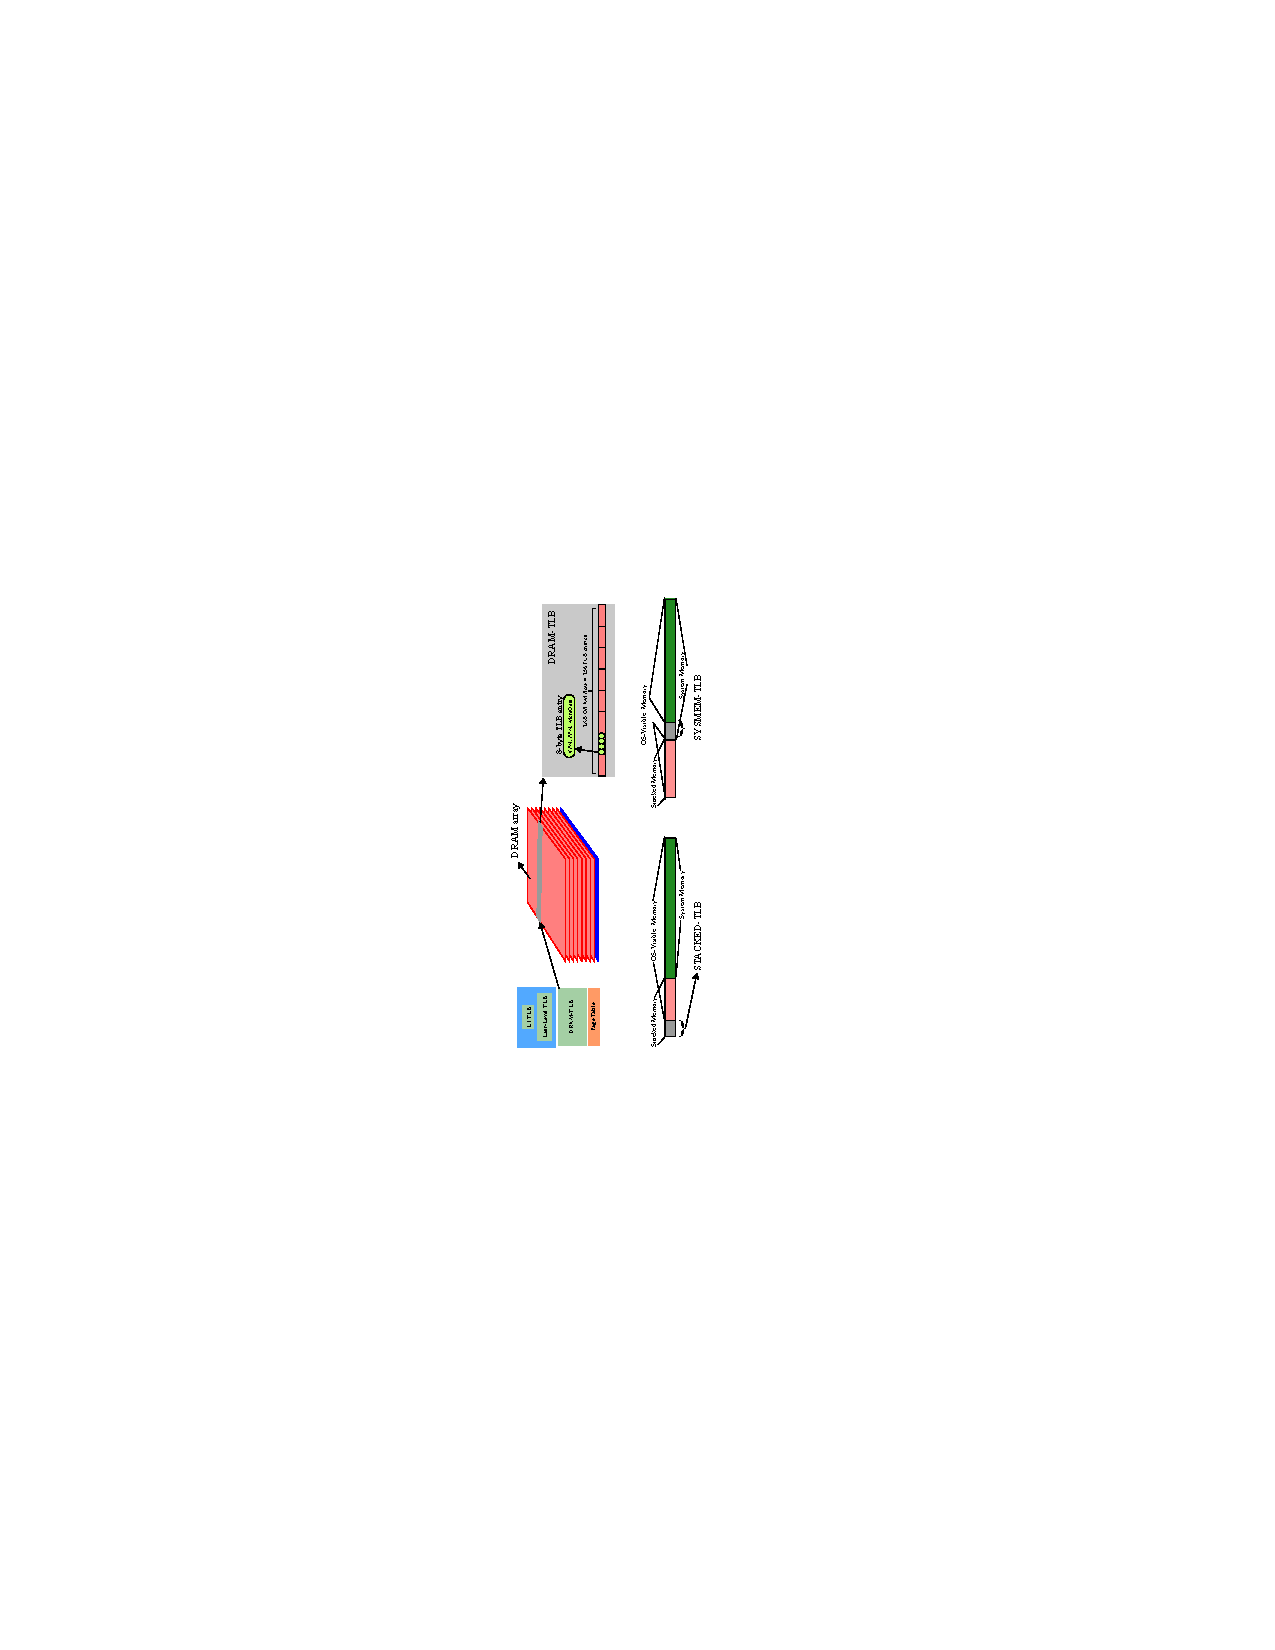
\psfig{file=FIGURES/stacked_tlb,angle=-90,width=\columnwidth}}
   \centerline{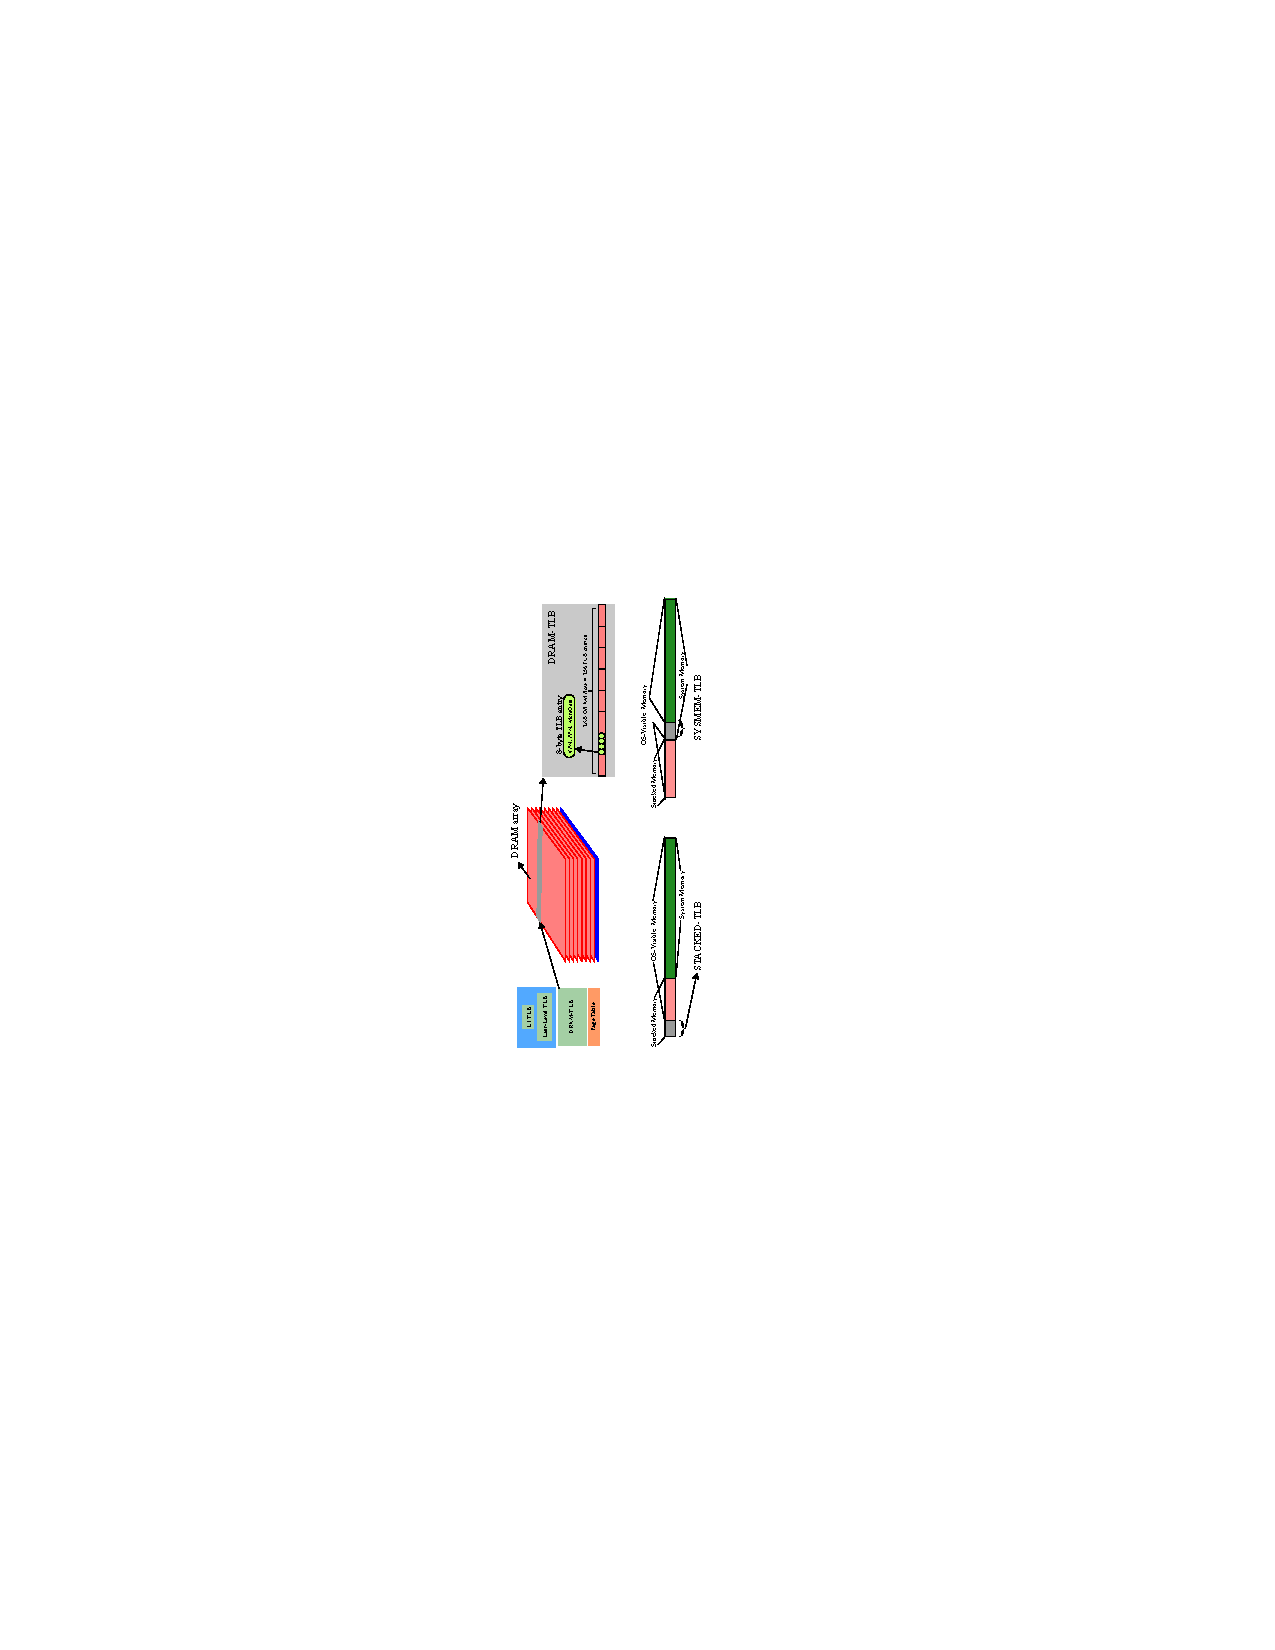
\psfig{file=FIGURES/stacked_tlb,width=\textwidth}}

  \caption{\small Improving TLB coverage by embedding TLBs in DRAM
    (DRAM-TLB). A DRAM-TLB architected using commodity DRAM is called
    SYSMEM-TLB and a DRAM-TLB architected with stacked DRAM is called
    Stacked-TLB. \normalsize}
  \label{fig:stacked_tlb} 
  \vspace{-0. in}
\end{figure*}


% For the workloads under study, we observe roughly 1.7 page table
% accesses per LLT miss. This translates to 30\% LLT misses requiring
% one page table lookup (PT) and 70\% requiring two page table lookups
% (PD and PT). This effectively means that roughly 65\% of the LLT
% misses are to the PT level. Thus, we propose {\em Distributed Memory
% Placement (DistrMemPlace)} where the commonly accessed PT level is
% always placed in stacked memory while the PML4, PDP, and PD levels are
% all placed in system memory (see
% Figure~\ref{fig:pagetable_placement}). In doing so, this placement
% policy provides higher bandwidth to the PT level. Doing so also has
% the benefit that requests that tend to be satisfied by more than one
% memory access (i.e. PD requests) do not contribute additional queueing
% delays to those requests that are satisfied by just one more memory
% access (i.e. PT requests and application memory requests).

Figure~\ref{fig:tlblat_placement} illustrates that distributed page
table placement further improves LLT miss latency by distributing page
table accesses in the hybrid memory system. Distributed Placement
reduces LLT miss latency on average by 40\%.
Figure~\ref{fig:perf_placement} shows that the reduction in LLT miss
latency helps improve workload performance further by an additional
14\%. Overall, distributed page table placement improves performance
on average by 28\% (up to 80\% for workloads like $BH$ and $BFS$).

% \subsection{Page Table Placement Analysis}

% These performance improvements can be correlated to the
% 5-40\% improvement in TLB miss latency (see
% Figure~\ref{fig:tlblat_placement}).

% We observe that increasing the memory traffic to stacked memory tends
% to increase the LLC miss latency by 10-20\%. This is to be expected
% due to increasing queuing delays in stacked memory. However, GPUs can
% tolerate cache miss latency fairly well~\cite{bwa}. There are a couple
% of outliers such as AMG\_1 and CoMD that seem to be sensitive to cache
% miss latency.

% In general, we observe that stacked memory placement of page tables in
% stacked memory tends to have similar (or worse) LLT
% load-to-use-latency relative to system memory placement of page
% tables. For example, DMR is sensitive to TLB miss latency hence sees
% performance degradation. The performance degradations for AMG\_1, is
% because the additional page table traffic to stacked memory causes a
% 40\% increase in average memory access latency (with little or no
% change in TLB miss latency). 

%\newpage
\subsection{Page Table Placement Discussion}

% \subsubsection{Storage Space}

\noindent The different page table placement policies clearly show a
correlation between LLT miss latency and system performance. We
observe that simple modifications to the page table placement policy
in a hybrid memory system can significantly improve the performance of
TLB-sensitive workloads. These performance improvements can be
realized without requiring any hardware changes.

Page table placement requires minor changes to the OS to allocate page
tables in stacked memory rather than system memory. The storage space
for the page table is a small fraction of the total capacity of
stacked memory. Recall that the page table storage overhead with 4KB
pages is only 0.2\% of the total application memory footprint. For
example, an application with 4GB of memory footprint requires only 8MB
of stacked memory space to store the page table.

% \subsubsection{Impact on CPU Performance}
% 
% In our baseline system, the latency to stacked memory and system
% memory is similar (e.g. on-die integrated heterogeneous CPU-GPU
% systems), and both StackedTLB and Distributed Placement do not impact
% CPU performance. Of the two, StackedTLB is the best performing because
% it is more bandwidth efficient than Distributed Placement. Remember
% that page tables are always placed in system memory (the baseline
% policy) when using StackedTLB.
% 
% StackedTLB does not impact CPU performance on systems where stacked
% memory latency is larger than system memory (e.g. heterogeneous
% systems with discrete GPUs). To ensure no impact on CPU performance,
% the CPU can always follow the baseline policy of walking the page
% table when it misses in its own last level TLB, rather than probing
% the StackedTLB. A dynamic decision may be possible where the CPU can
% adapt to either probing the StackedTLB or walking the page table
% depending on whether the average latency to StackedTLB is lower than
% the average latency of walking the page table in system memory.

% \subsubsection{Page Table Placement Limitations}

% \noindent While high performing, page table placement does not reduce
% the average number of memory accesses on an LLT miss. Consequently,
% the bandwidth required for address translation remains unchanged.
% Thus, it would be highly desirable to reduce the number of memory
% accesses on an LLT miss. Doing so not only improves memory access
% bandwidth but also reduces the effective LLT miss latency. The next
% section proposes such a technique by embedding another level of the
% TLB hierarchy in DRAM.

% To that end, the next
% section proposes to increase the coverage of the processor TLB
% hierarchy by architecting TLBs in DRAM.

% Long page table access latencies to system memory manifest because of
% two reasons. First, page table access traffic contends with existing
% memory access traffic that saturates system memory. Second, the LLT
% miss traffic alone can saturate

% due to the long queuing delays of the bandwidth bottlenecked system
% memory. 
